\documentclass[aps,prb,onecolumn,10pt,floatfix,superscriptaddress]{article} %pueden consultarse mas clases en 'REVTEX 4.1 Command and Options Summary'
%prb es la revista con las citas como superindices
%document class: article [twocolums,10pt,a4paper], book

\usepackage{listings}
\usepackage{amssymb} %amssymb y amsmath se usan juntos para ampliar
\usepackage{amsmath} %la cantidad de simbolos disponibles

\usepackage{graphicx} % permite usar imagenes fuera del modo dvi
\usepackage[spanish]{babel} % le dice al compilador que el idioma de escritura es espa\~nol
\usepackage[latin1]{inputenc} % permite usar caracteres de idiomas derivados del lat\'in
% \usepackage[T1]{fontenc} % permite usar acentos en el c\'odigo fuente

 \usepackage[pdftex,colorlinks=true,pdfstartview=FitH,linkcolor=blue,citecolor=blue,urlcolor=blue]{hyperref} % agrega hiperv\'inculos a la presentaci\'on en pdf

\usepackage[left=3cm,right=3cm,top=2cm,bottom=2cm]{geometry}
\renewcommand{\thefootnote}{\fnsymbol{footnote}}
%\usepackage[switch]{lineno} %Marca el n\'umero de linea... Poner \linenumbers donde se quiere empezar a contar
%\DeclareGraphicsExtensions{.pdf,.png,.jpg,.eps}%lo obvio

\begin{document}

\title{Pr\'actica $5$ : Aprendizaje no supervisado}

\author{Melisa Maidana Capit\'an}

\date{Junio 2013} % se puede utilizar \today para que ponga autom\'aticamente la fecha

\maketitle 
%\tableofcontents
% 

\setlength{\parindent}{30pt}
\setlength{\parskip}{2.5ex plus 0ex minus 0ex}

\section*{Resumen}

\section{Aprendizaje no supervisado}

La diferencia principal entre aprendizaje supervisado y aprendizaje no supervisado radica en el hecho de que en el segundo no hay realimentaci\'on a la red respecto a si las respuestas son o no correctas. La red debe descubrir por si misma patrones, caracter\'isticas, regularidades, correlaciones o categorias en los datos de entrada y codificarlos en las salidas. En cierta forma, las unidades y conexiones deben mostrar alg\'un grado de auto-organizaci\'on.

El aprendizaje no supervisado resulta \'util cuando hay redundancia en los datos de entrada a la red. El tipo de patr\'on que detecta una red de aprendizaje no supervisado depende de la estructura de la misma. Una red que aprende no supervisadamente puede decir cosas como

\begin{itemize}

\item Familiaridad : La red puede decir que tan parecido es un patr\'on nuevo, a otros aprendidos en el pasado. Progresivamente, la red va aprendiendo los nuevos patrones.

\item An\'alisis de componentes principales: Construye bases o ejes a lo largo de los cu\'ales los ejemplos presentados son similares a los anteriores. 

\item Agrupamiento o clustering :  Buscar patrones a partir de correlaciones en las entradas.

\item Feature Mapping : Si las salidas tienen una topolog\'ia determinada se pueden mapear las entradas a diferentes puntos de las salidas. Esto es arreglar una topograf\'ia para las entradas. Se espera que las salidas se auto-organicen.

\end{itemize}

\subsection{An\'alisis de componentes principales}

Se realiz\'o an\'alisis de componentes principales de una red de cuatro entradas y una salida. La salida dada por 

\begin{equation}
V = \sum^{4}_{j=1} \omega_{j}\xi_{j}
\end{equation}

con distribuci\'on de probabilidad de entradas dada por 

\begin{equation}
P(\bar{\xi}) = \frac{1}{(2\pi)^{2}(det(\Sigma))^{\frac{1}{2}}} exp(-\frac{1}{2}\bar{\xi^{T}}\Sigma^{-1}\bar{\xi})
\end{equation}

donde 

\begin{math}
\Sigma = 
\left(
  \begin{array}{cccc}
    2 & 1 & 1 & 1 \\
    1 & 2 & 1 & 1 \\
    1 & 1 & 2 & 1 \\
    1 & 1 & 1 & 2
  \end{array}
\right)
\end{math}

El aprendizaje se implemet\'o utilizando la regla de la Oja.

\begin{equation}
\Delta\omega_{j} = \eta V (\xi_{j}-V \omega_{j})
\end{equation}

La Fig.(\ref{apren1}) muestra los resultados obtenidos para los pesos asint\'oticos de la red, que son la direcci\'on principal de la matriz Sigma.

%==FIGURA======FIGURA======FIGURA======FIGURA======FIGURA======FIGURA=====
\begin{figure}[!htd] 
   	\begin{center}
   	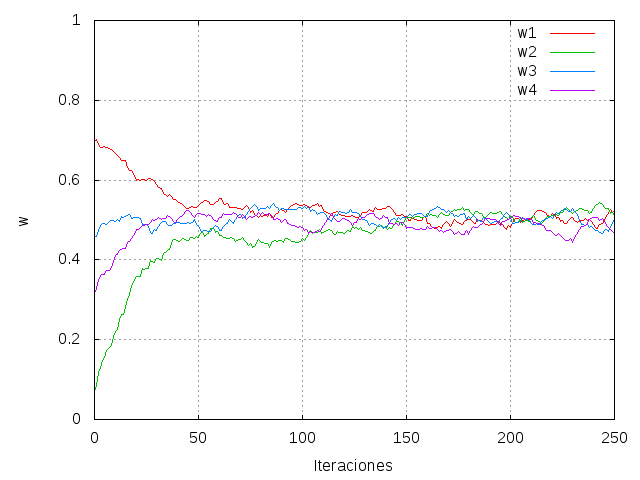
\includegraphics[scale=0.4 ]{apren1.png}
  \caption{\label{apren1} Valores asint\'oticos de los pesos que son similares a los valores del autovector correspondiente al autovalor m\'as grande de la matriz Sigma.}
    \end{center}
 \end{figure}
%==FIGURA======FIGURA======FIGURA======FIGURA======FIGURA======FIGURA=====

\subsection{Red neuronal de Kohonen: Feature Maping}

Se implement\'o una red neuronal de Kohonen con dos neuronas de entrada y diez neuronas de salida. Se aliment\'o a la red con una entrada con distribuci\'on 

\begin{equation}
P(\bar{\xi}) = 
\left\lbrace 
\begin{array}{l}
constante $ si r$ \in [0.9,0.11],\theta \in [0,\pi]\\
0 $ si no$   
\end{array}\right. 
\end{equation}

Adem\'as se utiliz\'o una funci\'on de vecindad gaussina dada por $exp^{-(i-i*)^{2}/2\sigma^2}$.

La idea de este algoritmo es lograr alg\'un tipo de organizaci\'on en las neuronas de salidas que corresponda con alguna caracter\'istica de las neuronas de entrada. En particular, el algoritmo "el ganador se lleva todo" aplicado a la arquitectura propuesta, lleva a que todos los pesos se organizacen tomando el valor del m\'as grande. El algoritmo elige un ganador, y modifica las vecindades del mismo. 

La Fig.(\ref{kohonen}) presenta los resultados obtenidos para la red de dos neuronas de entrada y diez de salida. Se presenta la evoluci\'on de los pesos para distinto numero de iteraciones, y para distintos valores de $\sigma$.
 
%==FIGURA======FIGURA======FIGURA======FIGURA======FIGURA======FIGURA=====
\begin{figure}[!htd] 
	\begin{minipage}[b]{0.450\linewidth}
	   	    \begin{center}
   	    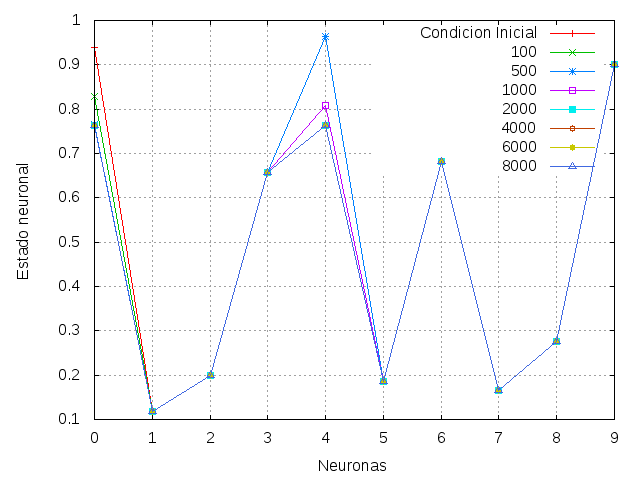
\includegraphics[scale=0.32 ]{sigma01_1.png}
     	    \end{center}
   \end{minipage}
   \begin{minipage}[b]{0.450\linewidth}
      	     \begin{center}
   	    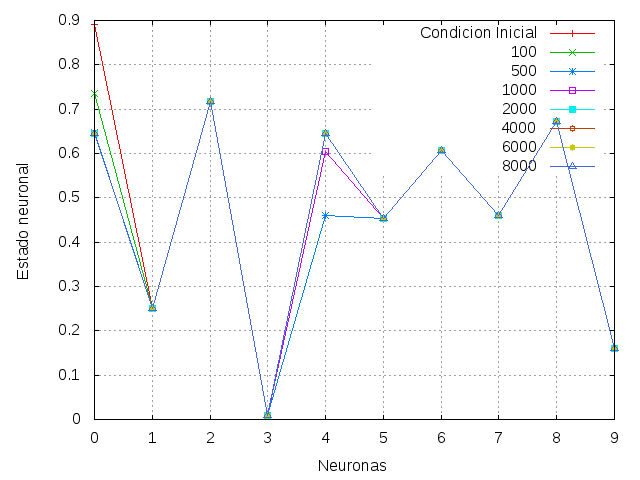
\includegraphics[scale=0.32 ]{sigma01_2.png}
     	    \end{center}
   \end{minipage} 
	\begin{minipage}[b]{0.450\linewidth}
	   	    \begin{center}
   	    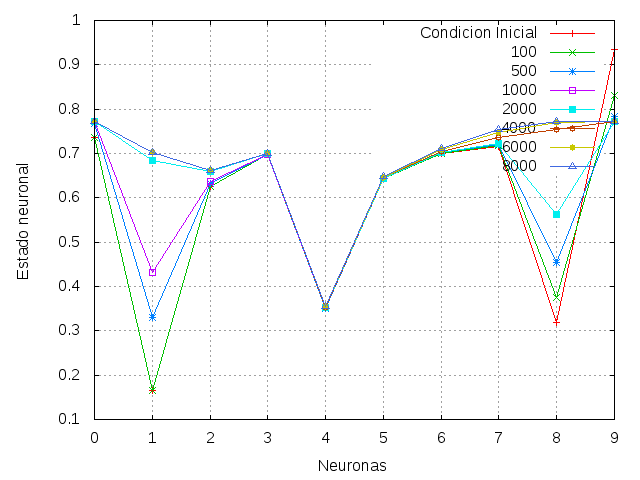
\includegraphics[scale=0.32 ]{sigma05_1.png}
     	    \end{center}
   \end{minipage}
   \begin{minipage}[b]{0.450\linewidth}
      	     \begin{center}
   	    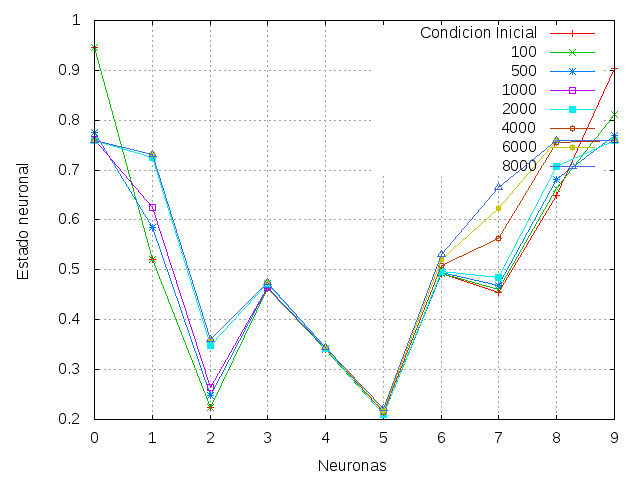
\includegraphics[scale=0.32 ]{sigma05_2.png}
     	    \end{center}
   \end{minipage} 
   	\begin{minipage}[b]{0.450\linewidth}
      	    \begin{center}
   	    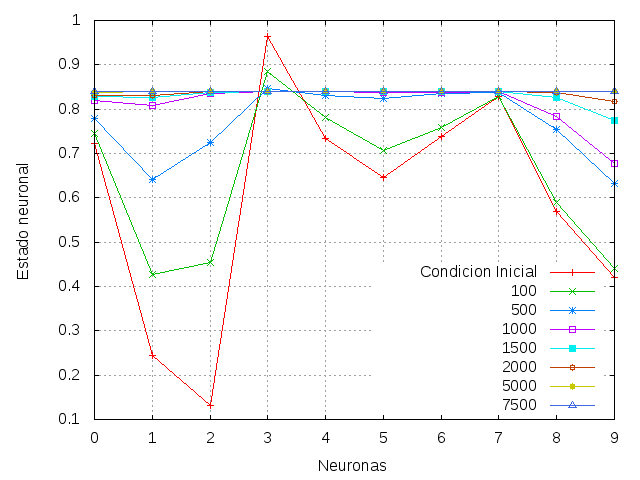
\includegraphics[scale=0.32 ]{sigma1_1.png}
     	    \end{center}
   \end{minipage}
   \begin{minipage}[b]{0.450\linewidth}
      	     \begin{center}
   	    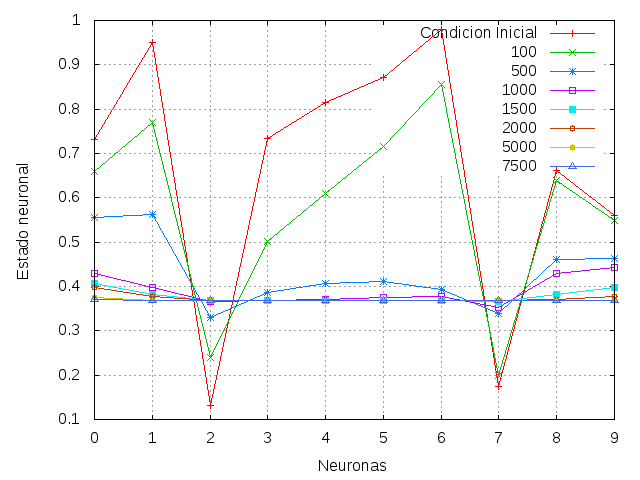
\includegraphics[scale=0.32 ]{sigma1_2.png}
     	    \end{center}
   \end{minipage}    
   
 \end{figure}
%==FIGURA======FIGURA======FIGURA======FIGURA======FIGURA======FIGURA=====

En la Fig.(\ref{kohonen}) se observa que para valores de sigma peque\~nos ($\sigma = 0.1$), los pesos de las neuronas lejanas al ganados no llegan a converguer a su valor, incluso para muchas iteraciones. Cuando aumenta el valor de $\sigma$, aumenta el entorno de influencia del ganador en sus vecino, de modo que afecta a vecinos m\'as lejamos. Por eso se ve en $\sigma = 2$ que luego de un n\'umero finito de iteraciones, todos los pesos se alinean en un valor, correspondiente al del ganador (el cu\'al se modifica muy poco en comparaci\'on de los dem\'as).

\subsection{Problema del viajante de comercio}

Se program\'o una red neuronal con dos neuronas de entrada y N neuronas de salida, donde la salida se encuentra dispuesta en topolog\'ia circular. Sin embargo, no se obtuvo un resultado razonable.

\section{Programas en C}

\subsection{An\'alisis de componentes principales}

\begin{lstlisting}[frame=single,breaklines=true]
#define PI 3.14159

void GeneraPatron(VecDoub &z);
void ProdMatVec(MatDoub &sigma,VecDoub &z);

int main(){
	
	int N_IN=4;
	double eta=0.01;

	VecDoub J(N_IN);
	VecDoub z(N_IN);
	MatDoub sigma(N_IN,N_IN);
	double v;

	for(int i=0;i<sigma.nrows();i++){
		for(int j=0;j<sigma.ncols();j++)
			sigma[i][j]=0.309;
		sigma[i][i]+=1;
		}

	srand(time(0));
	for(int i=0;i<J.size();i++)
		J[i]=rand()*1.0/RAND_MAX;

	double t=0;
	while(t<10000){
		v=0;
		GeneraPatron(z);
		ProdMatVec(sigma,z);
		for(int i=0;i<N_IN;i++)
			v+=J[i]*z[i];
		for(int i=0;i<N_IN;i++){
			J[i]+=eta*v*(z[i]-v*J[i]);
			}
		for(int i=0;i<N_IN;i++)
			cout << J[i] << endl;
		t++;
		}
	
	for(int i=0;i<N_IN;i++)
		cout << J[i] << endl;
		
	return 0;
	}
	
void GeneraPatron(VecDoub &z){
	
	double p;
	double sigma=1.0;
	double aleat;
	double r;
	int prueba;
	int n=z.size();
	
	for(int i=0;i<n;i++){
		prueba=0;
		while (prueba==0){
			aleat = rand()*1.0/RAND_MAX;
			p=exp(-aleat*aleat/2*sigma*sigma)/(sigma*2*PI);
			r=rand()*1.0/RAND_MAX;
			if(r<p)
				prueba=1;
			}
		z[i]=aleat;
		}
	}

void ProdMatVec(MatDoub &sigma,VecDoub &z){
	
	int n=z.size();
	VecDoub aux(n);
	for(int i=0;i<n;i++){
		aux[i]=0;
		for(int j=0;j<n;j++)
			aux[i]+=sigma[i][j]*z[j];
			}
	
	for(int i=0;i<n;i++)
		z[i]=aux[i];
	}
\end{lstlisting}

\subsection{Algoritmo de Kohonen}

\begin{lstlisting}[frame=single,breaklines=true]

void GeneraPatronUniforme(VecDoub &z);
double ProbPolar(VecDoub &z);
void InitWeigh(MatDoub &matrix);
void CalculoH(MatDoub &J,VecDoub &z,VecDoub &h);
int MaxVectorPosition(VecDoub &vec);
double Lambda(int i1,int i2,double sigma);
void CalculoDeltaJ(double eta,MatDoub &J,VecDoub &z,MatDoub &AJ,int winner,double sigma);
void ModificoPesos(MatDoub &pesos,MatDoub &delta);
	
int main(){

	int N_IN=2,N_OUT=10;
	double eta=0.01;
	double sigma=1;
	
	MatDoub J(N_OUT,N_IN);
	VecDoub z(N_IN);
	MatDoub AJ(N_OUT,N_IN);
	VecDoub h(N_OUT);
	double prob=0;
	
	srand(time(0));
	InitWeigh(J);
	
	while(prob==0){
		GeneraPatronUniforme(z);
		prob=ProbPolar(z);
		//cout << prob << endl;
	}
	FILE *datos;
	int winner;
	int tiempo=0;
	int tmax=10000;
	while(tiempo<tmax){
		CalculoH(J,z,h);
		if(tiempo%100==0){
		string output=to_string(tiempo)+to_string("_")+to_string(sigma)+to_string(".dat");
        if((datos = fopen(output.c_str(), "w")) == NULL){
            printf("No puedo abrir el archivo %s.\n", output.c_str());
            exit(1);
        }
		for(int i=0;i<J.nrows();i++){
			for(int j=0;j<J.ncols();j++)
				fprintf(datos,"%lf\t", J[i][j]);
				fprintf(datos,"\n");
				}
			}
		winner = MaxVectorPosition(h);
		CalculoDeltaJ(eta,J,z,AJ,winner,sigma);
		ModificoPesos(J,AJ);
	tiempo++;
	}
	
	return 0;

}

void GeneraPatronUniforme(VecDoub &z){
	int n=z.size();
    for(int i=0;i<n;i++)
		z[i]=rand()*1.0/RAND_MAX;
	}
	
double ProbPolar(VecDoub &z){
	
	int n=z.size();
	double r=0,theta;
	double p=0;
	
	for(int i=0;i<n;i++)
		r+=z[i]*z[i];
	r=sqrt(r);
	
	theta=atan(z[1]/z[0]);
	
	if(r>0.9 && r<1.1 && theta>0 && theta<atan(1))
		p=1;
	
	}
	
void InitWeigh(MatDoub &matrix){
	
	int n = matrix.nrows();
	int m = matrix.ncols();
	
	for(int i=0;i<n;i++){
		for(int j=0;j<m;j++){
			matrix[i][j] = rand()*1.0/RAND_MAX;
			}
		}
	}
	
void CalculoH(MatDoub &J,VecDoub &z,VecDoub &h){
	
	int n=J.nrows();
	//cout << "n=" << n << endl;
	int m=J.ncols();
	//cout << "m=" << m << endl;
	
	for(int i=0;i<n;i++){
		for(int j=0;j<m;j++){
			h[i]+=J[i][j]*z[j];
			}
		}
	}
	
int MaxVectorPosition(VecDoub &vec){
	
	int pos;
	int n=vec.size();
	double max;
	
	pos=0;
	max=vec[0];
	
	for(int i=0;i<n;i++){
		if(vec[i]>max){
			pos=i;
			max=vec[i];
			}
		}
	return pos;
	}

double Lambda(int i1,int i2,double sigma){
	
	double resultado;
	double exponente;
	
	exponente=(i1-i2)*(i1-i2);
	exponente=sqrt(exponente);
	
	resultado = exp(-exponente/(2*sigma*sigma));
	
	return resultado;
	}
	
void CalculoDeltaJ(double eta,MatDoub &J,VecDoub &z,MatDoub &AJ,int winner,double sigma){
	
	int n=J.nrows();
	int m=J.ncols();
	
	for(int i=0;i<n;i++)
		for(int j=0;j<m;j++)
			AJ[i][j]=eta*Lambda(i,winner,sigma)*(z[j]-J[i][j]);
	}
	
void ModificoPesos(MatDoub &pesos,MatDoub &delta){
	
	int n=pesos.nrows();
	int m=pesos.ncols();
	
	for(int i=0;i<n;i++)
		for(int j=0;j<m;j++)
			pesos[i][j]+=delta[i][j];

	}

\end{lstlisting}

\subsection{Problema del viajante de comercio}

\begin{lstlisting}[frame=single,breaklines=true]
void GeneraCoordenadas(MatDoub &mat);
void InitWeigh(MatDoub &matrix);
int MaxVectorPosition(VecDoub &vec);
void OrdenaVector(VecDoub &vector,MatDoub &mat);
double CalculoDistancia(const MatDoub &mat);
	
int main(){
	
	int N_IN=2,N_OUT;
	double alpha=0.8;
	
	for(N_OUT=50;N_OUT<=100;N_OUT++){
	
		double d = N_OUT;
		MatDoub J(N_OUT,N_IN);
		VecDoub z(N_IN);
		VecDoub angulo(N_OUT);
		VecDoub ord_ciudades(N_OUT);
		
		MatDoub ciudades(N_OUT,N_IN);
		GeneraCoordenadas(ciudades);
		
		for(int i=0;i<N_OUT;i++)
			angulo[i]=i*4*1.0*asin(1)/N_OUT;
		
		/*FILE *coordenadas;
		coordenadas=fopen("coordenadas.dat","w");
		for(int i=0;i<N_OUT;i++)
			fprintf(coordenadas,"%i\t%lf\t%lf\n",i,ciudades[i][0],ciudades[i][1]);*/
		
		srand(time(0));
		InitWeigh(J);
		
		int winner;
		int tiempo=0;	
		int tmax=1;	
		double d0=d;
		while(tiempo<=tmax){
			for(int i=0;i<ciudades.nrows();i++){
				VecDoub h(N_OUT);
				for(int k=0;k<N_OUT;k++){
					for(int j=0;j<N_IN;j++)
						h[k]+=J[k][j]*ciudades[i][j];
						/*if(tiempo==tmax && i==2)
							cout << h[k] << endl;*/
						}			
				winner = MaxVectorPosition(h);
				for(int k=0;k<N_OUT;k++){
					double dist = ((k-winner)%N_OUT);
					if(dist<=d){
						for(int j=0;j<N_IN;j++)
							J[k][j]= J[k][j] + alpha*(ciudades[i][j]-J[k][j]);
						}
					}
			if(tiempo==tmax){
				double prom_cos=0,prom_sin=0,prom=0;
				for(int j=0;j<N_OUT;j++){
					prom_cos+=h[j]*cos(angulo[j]);
					prom_sin+=h[j]*sin(angulo[j]);
					}	
				prom=atan2(prom_sin,prom_cos);
				if(prom<0)
					prom+=4*asin(1);
				ord_ciudades[i]=prom;
				}	
					
			}
			alpha-=0.01;
			d=d-(d0-1)/tmax;
			tiempo++;
		}
		
		OrdenaVector(ord_ciudades,ciudades);
		double distancia = CalculoDistancia(ciudades);
		cout << N_OUT << " " << distancia << endl;
	}

	return 0;
}

void GeneraCoordenadas(MatDoub &mat){
	
	int n=mat.nrows();
	int m=mat.ncols();
	
    for(int i=0;i<n;i++)
		for(int j=0;j<m;j++)
			mat[i][j]=rand()*1.0/RAND_MAX;
	}
	
void InitWeigh(MatDoub &matrix){
	
	int n = matrix.nrows();
	int m = matrix.ncols();
	
	for(int i=0;i<n;i++){
		for(int j=0;j<m;j++){
			matrix[i][j] = rand()*1.0/RAND_MAX;
			}
		}
	}
	
int MaxVectorPosition(VecDoub &vec){
	
	int pos;
	int n=vec.size();
	double max;
	
	pos=0;
	max=vec[0];
	
	for(int i=0;i<n;i++){
		if(vec[i]>max){
			pos=i;
			max=vec[i];
			}
		}
	return pos;
	}
	
void OrdenaVector(VecDoub &vector,MatDoub &mat){
	
	double a,x,y;
	int n=vector.size();
	
	for(int j=1;j<n;j++)
		for(int i=0;i<n-j;i++)
			if(vector[i]>vector[i+1]){
				a=vector[i+1];
				vector[i+1]=vector[i];
				vector[i]=a;
				x=mat[i+1][0];
				mat[i+1][0]=mat[i][0];
				mat[i][0]=x;
				y=mat[i+1][1];
				mat[i+1][1]=mat[i][1];
				mat[i][1]=y;
			}
	}
	
double CalculoDistancia(const MatDoub &mat){
	
	int n=mat.nrows();
	double dist=0;
	for(int i=0;i<n-1;i++)
		dist+=sqrt((mat[i][0]-mat[i+1][0])*(mat[i][0]-mat[i+1][0])+(mat[i][1]-mat[i+1][1])*(mat[i][1]-mat[i+1][1]));

	return dist;
	}


\end{lstlisting}


\begin{thebibliography}{99}

\bibitem IIntroduction to the theory of neural computation. John Hertz,Anders Krogh,Richard G.Palmer. Westview Press (1991).

\end{thebibliography}



\end{document}